\chapter{Coordinates.tex}

\section{Reference Orbit}

The ``Reference Orbit'' is the path of a ``reference'' particle that
is used to define a coordinate system for actual particles (particles
whose orbits are simulated in \bmad) as shown in
figure~\ref{f:local_coords}. At a given time $t$ the reference particle is
a distance $s = c \, t$ along the Reference Orbit from the Reference
Orbit zero position. The local $(x, y, z)$ coordinate system is such
that the origin is at the reference particle with the $z$--axis
parallel to the local reference orbit pointing in the direction of the
reference particle motion. The $x$ and $y$--axes are perpendicular to
the Reference Orbit. Typically the $y$--axis is in the vertical
direction and $x$--axis defines the horizontal direction.

\begin{figure}[tb]
\centering
\includegraphics{local_coords.ps}
\caption{The Local Reference System}
\label{f:local_coords}
\end{figure}

In \bmad\ a lattice is comprised of a sequence of elements: Quadrupoles,
bends, etc. Each element has an entrence point and an exit point and a
reference curve between them. For a bend the reference curve is
circular and for all other elements the reference curve is a straight
line. The elements are assembled together so that the exit point of
one element lies on top of the entrence point of the next with the
reference curves forming a smooth arc (no kinks). The Reference Orbit
is then just the sum of the reference curves. 

Notice that in a wiggler the reference orbit, which is a straight
line, does {\em not} correspond to the orbit that any actual particle
could travel. Typically the physical entity of an element is centered
about the reference curve but in general this may not be so. For
example, by specifying offsets and pitches, the centerline of a
quadrupole magnet may be arbitrarily oriented with respect to its
reference curve. Since the reference curve is fixed to the reference
curves of the preceding and following elements it is the physical
magnet that moves and not the reference curve. Notice in this case a
shifting of the physical magnet means that the reference curve does
{\em not} correspond to the orbit that any actual particle could
travel.


\section{Global Reference System}

\bmad, following the MAD convention, uses a Cartesian coordinate system
$(X, Y, Z)$ to describe the the position of the Reference orbit along
with three angles $\theta, \phi, \psi$ used to define an Reference
Orbit's orientation as shown in figure~\ref{f:global_coords}. Typically
(although there is nothing in \bmad\ that necessitates this) $Y$ is the
vertical coordinate and $(X, Z)$ are the ``floor'' coordinates. 
The definition of the three angles is:
\begin{description}
\item[$\theta$] Azimuth angle: Angle in the $(X, Z)$ plane 
between the $Z$--axis and the projection of the $z$--axis onto the
$(X, Z)$ plane. A positive angle of $\theta = \pi/2$ corresponds to the
projected $z$ axis pointing in the positive $X$ direction.
\item[$\phi$] Pitch (elevation) angle: Angle between the $s$--axis 
and the $Y$--axis. A positive angle of $\phi = \pi/2$ corresponds to
the $s$--axis pointing in the positive $Y$ direction.
\item[$\psi$] Roll angle: Angle of the $x$--axis with respect 
to the intersection of the $(X, Z)$ plane with the $(x, y)$ plane. A
positive $\psi$ forms a right--handed scew with the $s$--axis.
\end{description}

\begin{figure}
\centering
\includegraphics{global_coords.ps}
\caption{The Global Reference System}
\label{f:global_coords}
\end{figure}

By default at the Reference Orbits $s = 0$ point coincides with the
$(X, Y, Z)$ origin and at $s = 0$ the $x$, $y$, and $z$ axes
correspond to the $X$, $Y$, and $Z$ axes respectively. Positive
bending angle for horizontal bends result in negative $\theta$ which
corresponds to $x$ pointing radially outward. Without any vertical
bends the $Y$ and $y$ axes will coinside with $\phi = \psi = 0$. 

\section{Phase Space Coordinate System}

The canonical phase space coordinates that \bmad\ uses for tracking a
particle is $(x, p_x, y, p_y, z, p_z)$. $x$, $y$, and $z$ are the
coordinates with respect to the reference particle. $p_x$ and $p_y$
are the normalized momentum
\begin{align}
  p_x = &\frac{P_x}{P_0} \\
  p_y = &\frac{P_y}{P_0}
\end{align}
where $P_x$ and $P_y$ are the momentum components along the $x$ and
$y$ axes respectively and $P_0$ is the reference (sometimes called the
design) momentum. The longitudinal canonical momentum $p_z$ is given by
\begin{equation}
  p_z = \frac{\Delta E}{E_0}
\end{equation}
Where $E_0$ is the reference energy and $\Delta E = E - E_0$ is the
deviation of the particle's energy from the reference energy. MAD uses
a slightly different coordinate system. With MAD $(z, p_z)$ is
replaced by $(-c\Delta t, p_t = \Delta E / P_0 c)$. where $\Delta t$
is the time difference for a particle to pass a point relative to the
reference particle. For highly relativistic particles the two
coordinate systems are the same. For non-relativistic particles \bmad\
is not to be trusted in any case. \bmad\ generally uses the small angle
(paraxial) approximation where it is assumed that $p_x, p_y \ll 1$. With this
approximation the relationship between the cononical momenta and the
slopes $x' = dx/ds$ and $y' = dy/ds$ is
\begin{align}
  x' &\approx \frac{p_x}{1 + p_z} (1 + g x) \\
  y' &\approx \frac{p_y}{1 + p_z} (1 + g x) 
\end{align}
where $g = 1/\rho$ is the curvature function. $\rho$ being the radius
of curvature of the reference orbit. $g = 0$ in a straight section.

For those programmers using the PTC software package directly (ignore
this if you don't know what I'm talking about) \'Etienne Forest uses a still
different coordinate system. with PTC $(z, p_z)$ is replaced by
$(\Delta E/P_0 c, c \Delta t)$